\section{Esercizio 12 -- Esame di dicembre 2024}
\subsection{Progettazione}
Il sistema è composto da 2 nodi, A e B, che comunicano mediante handshaking. A legge i dati da una ROM e li invia uno alla volta a B, che somma progressivamente le stringhe ricevute utilizzando un sommatore e memorizza il risultato in un registro.

Uno schema a blocchi del sistema completo potrebbe essere quello in [Figura \ref{fig_december_exam_block_diagram}]

\begin{figure}[h]
    \centering
    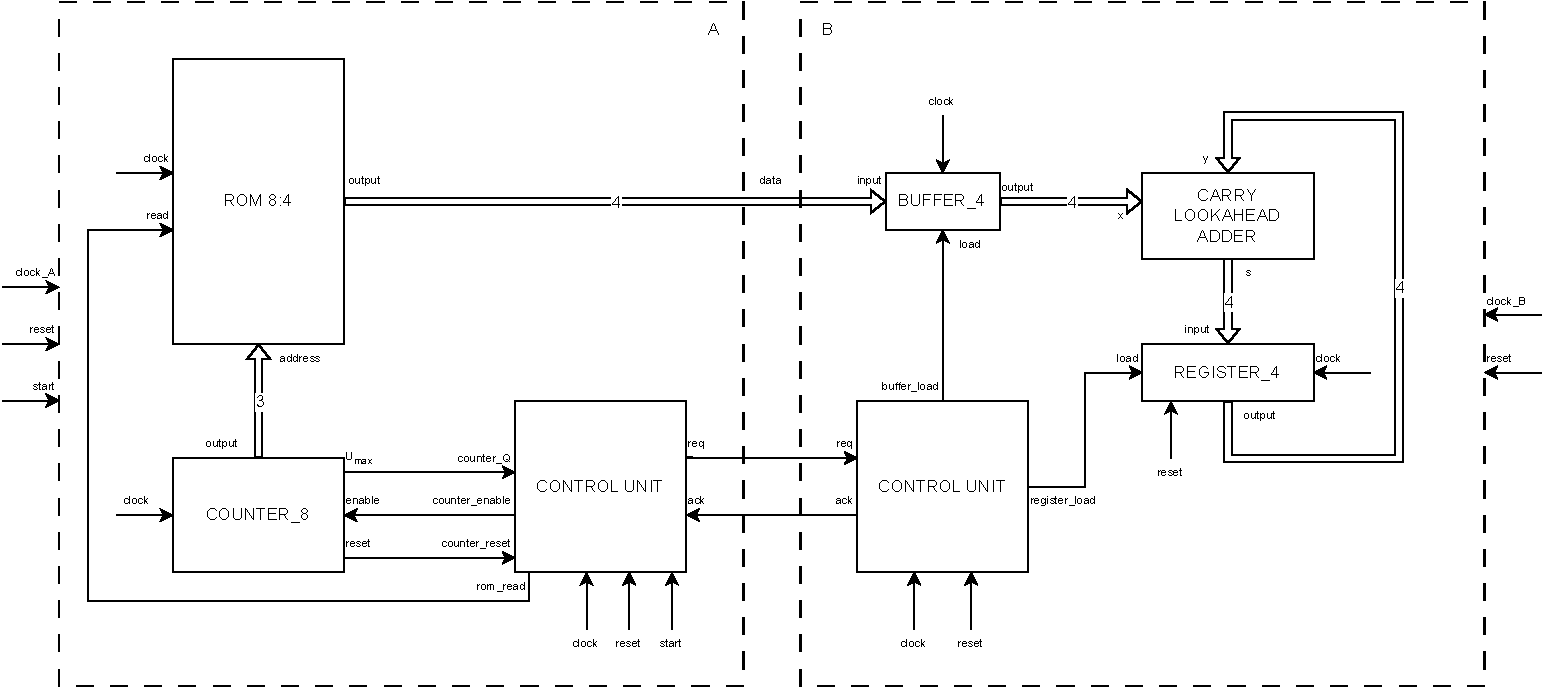
\includegraphics[width=\linewidth]{img/december_exam_block_diagram.pdf}
    \caption{Schema a blocchi del sistema complessivo}
    \label{fig_december_exam_block_diagram}
\end{figure}

Si fanno le seguenti assunzioni:

\begin{itemize}
    \item Sia la parte di controllo (le due control unit) che la parte operativa (le restanti parti dei sistemi) operano sul fronte di salita dei rispettivi clock;
    \item Tutti i registri e la ROM lavorano in maniera sincrona con il fronte di salita del proprio clock;
    \item I contatori alzano il segnale \texttt{Q} sul fronte di salita del proprio clock quando si azzerano;
    \item I segnali di reset (supposti in comune) abbassano anche tutte le uscite;
    \item I componenti di B sono inizializzati a zero.
\end{itemize}

Si riportano gli automi dei due sistemi [Figura \ref{fig:december_exam}]; a sinistra quello del sistema A, a destra quello di B.

\begin{figure}[h]
    \centering
    \begin{minipage}[c]{0.45\linewidth}
        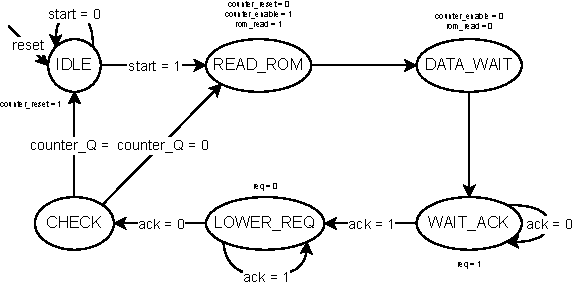
\includegraphics[width=\linewidth]{img/december_exam_A.pdf}
    \end{minipage}
    \hfill
    \begin{minipage}[c]{0.45\linewidth}
        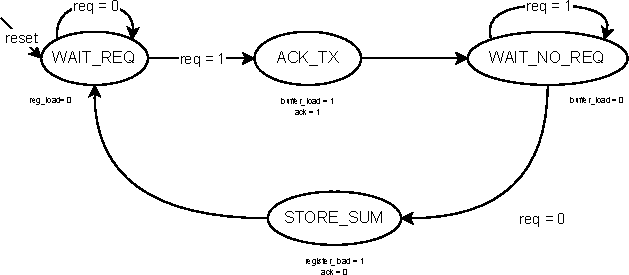
\includegraphics[width=\linewidth]{img/december_exam_B.pdf}
    \end{minipage}
    \caption{Automi dei sistemi A e B}
    \label{fig:december_exam}
\end{figure}

Si progetta il sommatore carry lookahead come mostrato in [Figura \ref{fig:carry_lookahead_adder_4}]. Si tratta di un sommatore a 4 bit, con i segnali di carry in ingresso e di carry out in uscita.

\begin{figure}[h]
    \centering
    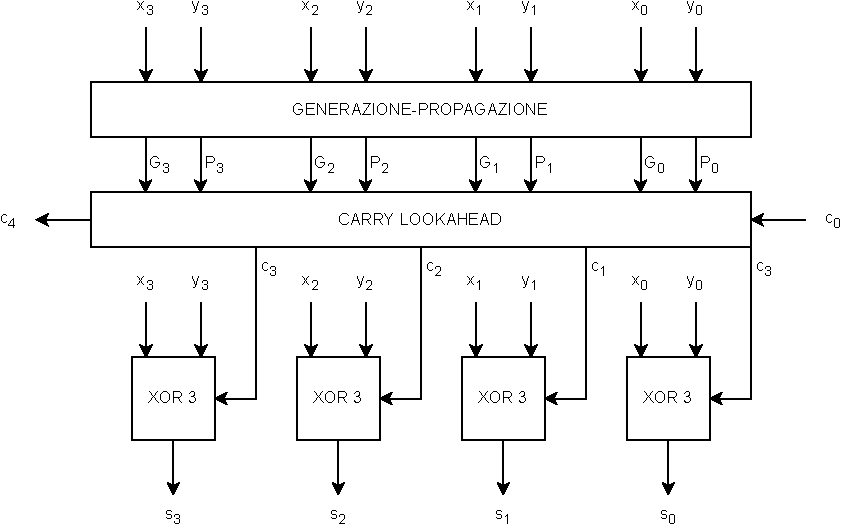
\includegraphics[width=0.5\linewidth]{img/carry_lookahead_adder_4.pdf}
    \caption{Schema a blocchi del sommatore carry lookahead a 4 bit}
    \label{fig:carry_lookahead_adder_4}
\end{figure}

Sia il blocco di generazione-propagazione che il blocco di carry lookahead sono composti da semplici porte AND e OR. Il vantaggio di questo tipo di sommatore è la possibilità di calcolare il carry in uscita senza dover attendere il carry in ingresso, riducendo così il tempo di propagazione del segnale.

Per semplicità, si riportano solo le espressioni logiche che esprimono l'architettura dei due blocchi:

\begin{align*}
    G_i &= x_i \cdot y_i \\
    P_i &= x_i + y_i \\
    c_1 &= G_0 + P_0 \cdot c_0 \\
    c_2 &= G_1 + P_1 \cdot c_1 &= G_1 + P_1 \cdot G_0 + P_1 \cdot P_0 \cdot c_0 \\
    c_3 &= G_2 + P_2 \cdot c_2 &= G_2 + P_2 \cdot G_1 + P_2 \cdot P_1 \cdot G_0 + P_2 \cdot P_1 \cdot P_0 \cdot c_0 \\
    c_4 &= G_3 + P_3 \cdot c_3 &= G_3 + P_3 \cdot G_2 + P_3 \cdot P_2 \cdot G_1 + P_3 \cdot P_2 \cdot P_1 \cdot G_0 + P_3 \cdot P_2 \cdot P_1 \cdot P_0 \cdot c_0
\end{align*}

\subsection{Trascrizione in VHDL}
Si procede ora alla trascrizione del progetto in codice VHDL. Si riportano gli schemi a blocchi effettivi dei due sistemi [Figura \ref{fig:12_DECEMBER_EXAM}].

\begin{figure}[h]
    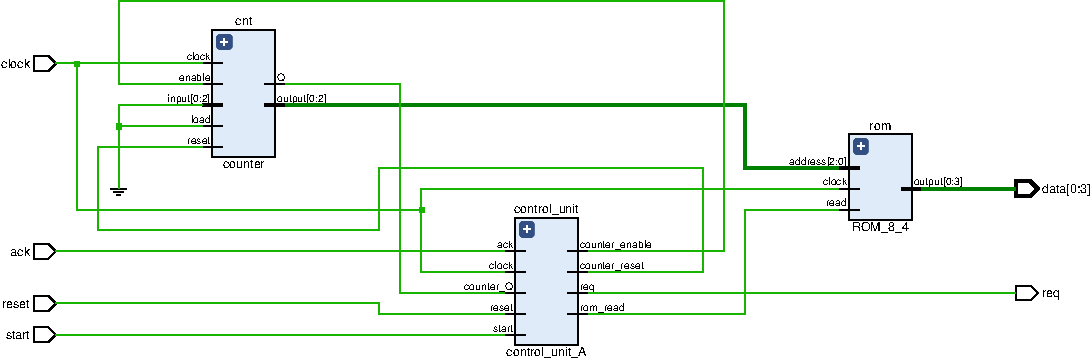
\includegraphics[width=\linewidth]{img/12_DECEMBER_EXAM_A.pdf}
    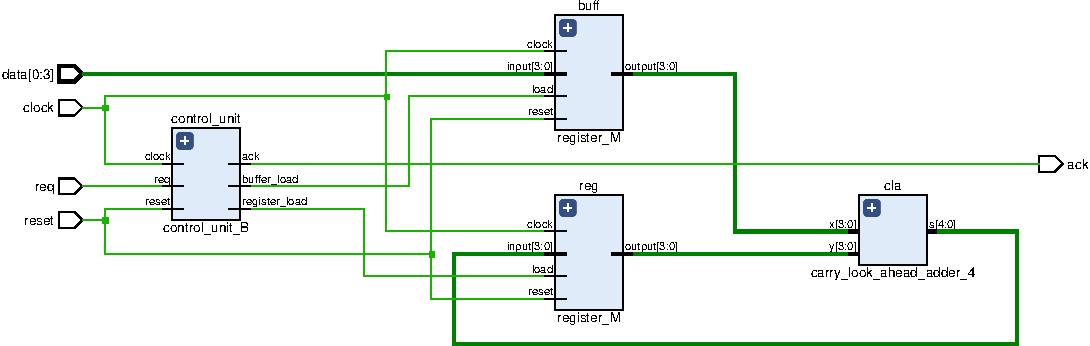
\includegraphics[width=\linewidth]{img/12_DECEMBER_EXAM_B.pdf}
    \caption{Schema a blocchi del sistema complessivo}
    \label{fig:12_DECEMBER_EXAM}
\end{figure}

\subsubsection{Implementazione}
In prima battuta si analizza il sistema A:

\begin{code}
    \inputminted{vhdl}{vhdl/december_exam_system_A.vhd}
    \caption{Implementazione del sistema A}
    \label{cod:december_exam_system_A}
\end{code}

\begin{code}
    \inputminted{vhdl}{vhdl/december_exam_control_unit_A.vhd}
    \caption{Implementazione dell'unità di controllo del sistema A}
    \label{cod:december_exam_control_unit_A}
\end{code}

\paragraph{Funzionamento generale.}
Il nodo A legge progressivamente i dati contenuti nella sua memoria ROM di 8 locazioni di 4 bit facendo uso di un contatore modulo 8. Alla lettura di ogni dato, esso invia il contenuto della locazione letta al nodo B mediante handshaking.

I componenti principali del nodo a sono:

\begin{enumerate}
    \item \texttt{control\_unit\_A}: unità di controllo del nodo A, coordina le operazioni dell'unità operativa;
    \item \texttt{ROM\_8\_4}: memoria ROM di 8 locazioni da 4 bit contenente i dati da inviare al nodo B;
    \item \texttt{counter\_mod\_8}: contatore modulo 8, consente la scansione della ROM fornendo ad essa l'indirizzo, equivalente al conteggio attuale.
\end{enumerate}

Nel dettaglio, il nodo A funziona nel seguente modo:

\begin{itemize}
    \item Il sistema si trova in uno stato di riposo fino all'arrivo di un segnale di \texttt{start};
    \item Il nodo A legge il contenuto della locazione di memoria ROM indicata dal contatore modulo 8, inizialmente posto a 0;
    \item Il contatore viene abilitato al conteggio per un ciclo di clock, affinché punti alla locazione successiva;
    \item Nel frattempo, il nodo A invia il dato letto al nodo B mediante handshaking, alzando \texttt{req};
    \item Il nodo A si mette in attesa di un segnale di \texttt{ack} da parte di B;
    \item Il processo viene ripetuto finché il contatore non raggiunge il valore massimo, dopodiché il sistema torna in uno stato di riposo.
\end{itemize}

\paragraph{Struttura del codice.}
L'architettura del sistema A è \texttt{structural} [Codice sorgente \ref{cod:december_exam_system_A}], essendo composto da sottoblocchi interconnessi tra loro. In particolare, i componenti utilizzati sono:

\begin{itemize}
    \item \texttt{control\_unit\_A} [Codice sorgente \ref{cod:december_exam_control_unit_A}]: coordina le operazioni dell'unità operativa e gestisce l'handshaking:
    \begin{enumerate}
        \item Il segnale di \texttt{start} fa partire il sistema;
        \item Il segnale di \texttt{req} viene alzato per richiedere l'invio di un dato a B;
        \item Il segnale di \texttt{ack} viene letto per confermare la ricezione del dato da parte di B;
        \item \texttt{counter\_enable} abilita il contatore per scansionare le locazioni della ROM;
        \item \texttt{counter\_reset} pone il conteggio a zero se la macchina è in uno stato di riposo;
        \item \texttt{counter\_Q} si alza quando il contatore ha superato il valore massimo e si è azzerato;
        \item \texttt{rom\_read} indica alla ROM di leggere il dato contenuto nella locazione indicata dal contatore.
    \end{enumerate}
    \item \texttt{ROM\_8\_4} [Codice sorgente \ref{cod:ROM_8_4}]: memoria ROM di 8 locazioni da 4 bit contenente i dati da inviare al nodo B:
    \begin{enumerate}
        \item \texttt{read} è un segnale di controllo, quando è alto la ROM legge il dato contenuto nella locazione puntata da \texttt{address};
        \item \texttt{address} rappresenta indirizzo della locazione da leggere;
        \item \texttt{output} contiene dato letto dalla ROM.
    \end{enumerate}
    \item \texttt{counter\_mod\_8} [Codice sorgente \ref{cod:counter_risingedge}]: contatore modulo 8, consente la scansione della ROM fornendo ad essa l'indirizzo, equivalente al conteggio attuale:
    \begin{enumerate}
        \item \texttt{enable} abilita il conteggio;
        \item \texttt{output} fornisce il valore attuale del conteggio;
        \item \texttt{Q} si alza quando il contatore ha superato il valore massimo e si è azzerato.
    \end{enumerate}
\end{itemize}

A questo punto si analizza il sistema B:

\begin{code}
    \inputminted{vhdl}{vhdl/december_exam_system_B.vhd}
    \caption{Implementazione del sistema B}
    \label{cod:december_exam_system_B}
\end{code}

\begin{code}
    \inputminted{vhdl}{vhdl/december_exam_control_unit_B.vhd}
    \caption{Implementazione dell'unità di controllo del sistema B}
    \label{cod:december_exam_control_unit_B}
\end{code}

\paragraph{Funzionamento generale.}
Il nodo B riceve i dati inviati da A e li somma progressivamente, memorizzando il risultato in un registro:

\begin{itemize}
    \item Il sistema si trova in uno stato di attesa fino all'arrivo di un segnale di \texttt{req};
    \item Il nodo B legge il dato inviato da A e lo carica in un registro di buffer;
    \item Il nodo B invia un segnale di \texttt{ack} ad A per confermare la ricezione del dato, e attende che \texttt{req} venga abbassato;
    \item Nel frattempo, il dato contenuto nel buffer viene sommato al contenuto precedente del registro tramite un sommatore di tipo carry look ahead e memorizzato nel registro stesso;
    \item Il processo viene ripetuto in maniera indefinita, tornando sempre in attesa di una comunicazione da parte di A.
\end{itemize}

\paragraph{Struttura del codice.}
L'architettura del sistema B è anch'essa \texttt{structural} [Codice sorgente \ref{cod:december_exam_system_B}]. Questa volta i sottoblocchi utilizzati sono:

\begin{itemize}
    \item \texttt{control\_unit\_B} [Codice sorgente \ref{cod:december_exam_control_unit_B}]: coordina le operazioni dell'unità operativa e gestisce l'handshaking:
    \begin{enumerate}
        \item Il segnale di \texttt{req} viene letto per ricevere un dato da A;
        \item Il segnale di \texttt{ack} viene alzato per confermare la ricezione del dato;
        \item \texttt{buffer\_load} carica il dato ricevuto in un registro di buffer;
        \item \texttt{register\_load} abilita il registro alla lettura con un'opportuna tempificazione, memorizzando la somma attuale ma mantenendo in uscita il dato precedente per il ciclo di clock corrente;
    \end{enumerate}
    \item \texttt{carry\_look\_ahead\_adder\_4} [Codice sorgente \ref{cod:carry_look_ahead_adder_4}]: sommatore carry lookahead a 4 bit:
    \begin{enumerate}
        \item \texttt{x} e \texttt{y} sono i due addendi;
        \item \texttt{s} restituisce la somma dei due addendi:
    \end{enumerate}
    \item \texttt{register\_M} [Codice sorgente \ref{cod:register_M}]: registro di 4 bit:
    \begin{enumerate}
        \item \texttt{load} segnale di controllo che abilita il caricamento del dato in input nel registro;
        \item \texttt{input} contiene il dato da caricare nel registro;
        \item \texttt{output} rispecchia il dato attualmente presente nel registro.
    \end{enumerate}
\end{itemize}

\subsubsection{Simulazione}
Si riporta il codice di test per la simulazione del sistema:

\begin{code}
    \inputminted{vhdl}{vhdl/december_exam_system_tb.vhd}
    \caption{Testbench per la simulazione del sistema}
    \label{cod:december_exam_system_tb}
\end{code}

Il testbench simula il comportamento del sistema A e B, verificando che i dati inviati da A vengano sommati correttamente da B. L'entity dichiarata all'inizio è vuota, in quanto il testbench non riceve input dall'esterno né fornisce alcun output.

\paragraph{Struttura del testbench.}
Il testbench è strutturato in questo modo:

\begin{enumerate}
    \item Dichiarazione dei componenti: il testbench crea un'istanza dei nodi A e B:
    \begin{itemize}
        \item \texttt{sys\_A}:
        \begin{itemize}
            \item Trasmette le stringhe contenute nella ROM, una alla volta;
            \item Alza il segnale di request ed attende l'acknowledgement da B prima di inviare il dato successivo.
        \end{itemize}
        \item \texttt{sys\_B}:
        \begin{itemize}
            \item Riceve i dati inviati da A e manda un ack per confermare la ricezione;
            \item Somma progressivamente i dati ricevuti;
            \item Memorizza il risultato in un registro.
        \end{itemize}
    \end{itemize}
    \item Dichiarazione dei segnali: vengono dichiarati i segnali di test utilizzati in simulazione:
    \begin{itemize}
        \item \texttt{CLK\_period\_A} e \texttt{CLK\_period\_B}: periodi di clock per i nodi A e B, modificati durante la simulazione;
        \item \texttt{clock\_A} e \texttt{clock\_B}: segnali di clock per i nodi A e B;
        \item \texttt{reset}: segnale di reset per i nodi A e B;
        \item \texttt{start}: segnale di controllo per avviare il sistema A;
        \item \texttt{req}, \texttt{data} e \texttt{ack}: segnali di handshaking tra i nodi A e B;
    \end{itemize}
    \item Definizione dei processi:
    \begin{itemize}
        \item \texttt{CLK\_A\_process} e \texttt{CLK\_B\_process}: generano i segnali di clock per i nodi A e B rispettivamente;
        \item \texttt{test\_process}: modifica i segnali di controllo per verificare il comportamento del sistema:
        \begin{itemize}
            \item \texttt{CLK\_period\_A} è impostato inizialmente a 10 ns, \texttt{CLK\_period\_B} a 23 ns;
            \item Si attendono 100 ns, si alzano prima \texttt{reset} e poi \texttt{start} per 25 ns così da avviare il sistema A e la comunicazione con B;
            \item Si attendono 1200 ns per completare un ciclo di funzionamento di A, si può osservare la correttezza del sistema quando il clock di A è maggiore di quello di B;
            \item Si scambiano i periodi di clock di A e B, si alzano nuovamente prima \texttt{reset} e poi \texttt{start} per 25 ns;
            \item Si attendono 400 ns per osservare che A comincia da capo il ciclo di funzionamento, mentre B riprende la somma con il valore del registro risalente all'ultima somma del ciclo precedente.
            \item Si fornisce un segnale di \texttt{reset} per terminare prematuramente il ciclo e si osserva l'imediata terminazione del ciclo di A e il ritorno allo stato di attesa con registro azzerato di B.
            \item Si attendono 100 ns e si forniscono un'ultima volta i segnali di \texttt{reset} e di \texttt{start} per 25 ns, per poi attendere indefinitamente. Si può osservare la correttezza del sistema quando il clock di A è minore di quello di B.
        \end{itemize}
    \end{itemize}
\end{enumerate}


\begin{figure}[h]
    \centering
    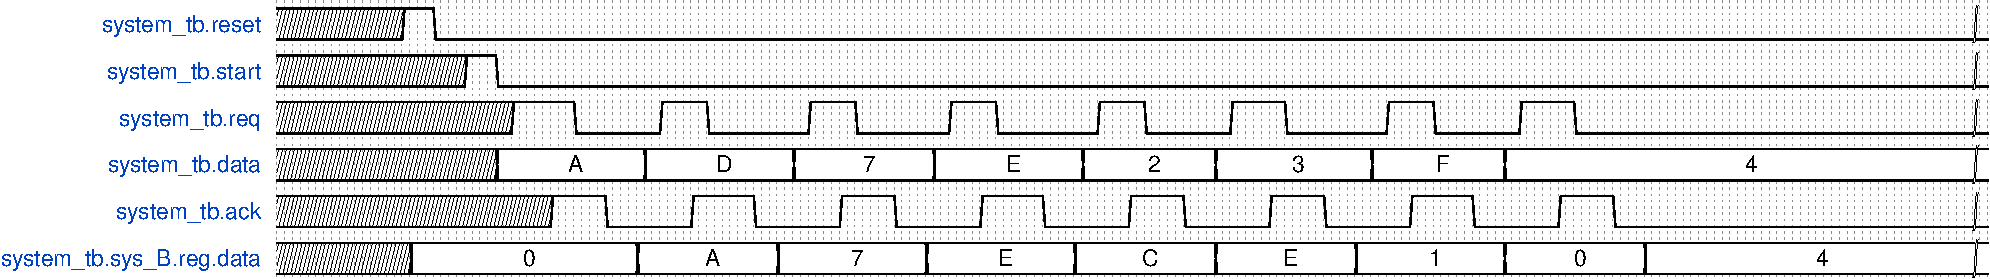
\includegraphics[width=0.75\linewidth]{img/december_exam_tb_1.pdf}
    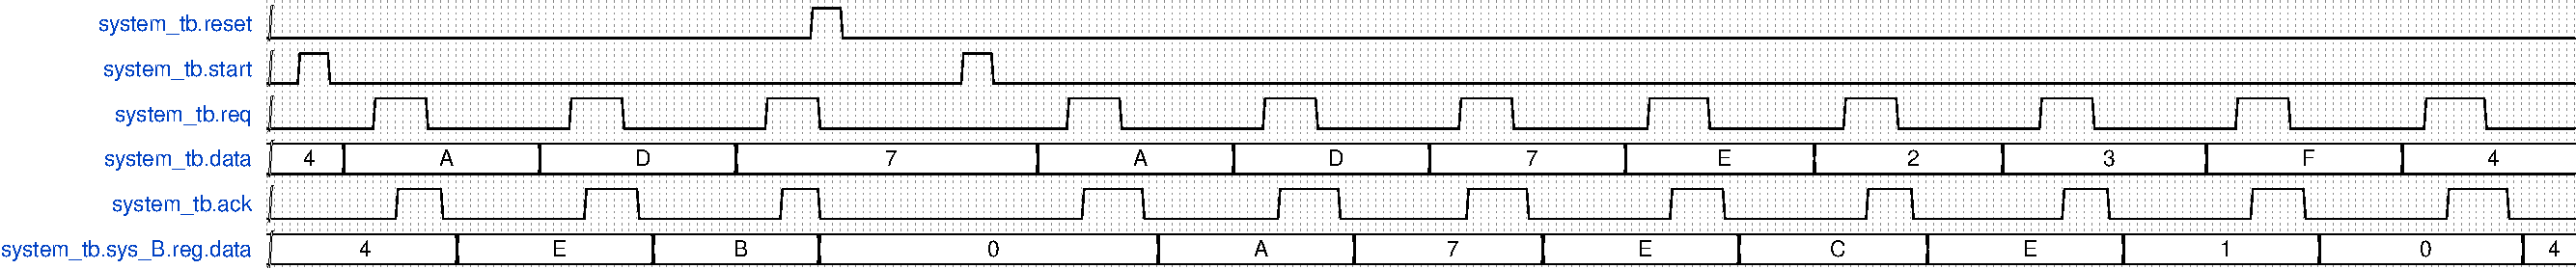
\includegraphics[width=\linewidth]{img/december_exam_tb_2.pdf}
    \caption{Simulazione del sistema}
    \label{fig:december_exam_tb}
\end{figure}
